\section{Simulation}
\rhead{Simulation}

Der erste Schritt ist ein Modell zu erstellen.
Dazu wird der Golfstrom in drei Zonen aufgeteilt. Die jeweiligen Polarregionen und der Äquator werden je zu eine Zone. Diese Zonen erhalten dann je eine Box.
Im laufe des Seminars wurden zwei Modelle erstellt. Der erste Ansatz war sehr lehrreich hatte aber  schlussendlich nichts mit dem realen Golfstrom gemeinsam. Der zweite Ansatz war erfolgreicher und der Golfstrom kann mit diesem Modell qualitativ simuliert werden.
In den folgenden zwei Kapiteln werden diese zwei Modelle vorgestellt und die jeweiligen Resultate diskutiert.

\subsection{Zwei-Fluss Modell( 1. Ansatz)}

In diesem Modell werden die Boxen jeweils durch Rohre verbunden wie im 2-Box Modell. Nun werden jedoch zwei Flüsse simuliert, die von den jeweiligen Dichtegradienten der unterschiedlichen Boxen abhängen. $q_1$ ist also nur vom Dichteunterschied zwischen Box $1$ und Box $2$ abhängig. Dementsprechend hängt auch $q_2$ nur vom Dichteunterschied der Boxen $2$ und $3$ ab.
Der Vorteil der Aufteilung der Flüsse ist, dass wir sie entkoppeln können und sie nicht von der jeweiligen dritten Box abhängig sind.
Eine Darstellung des Modelles ist in Abbildung 9.4 zu finden.

\begin{figure}
	\centering
	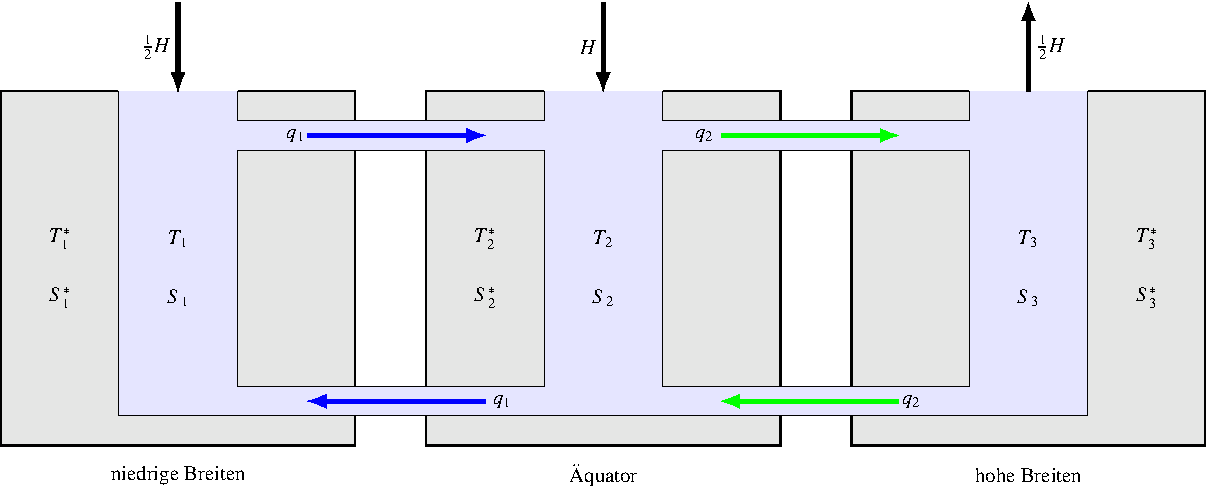
\includegraphics[width=14cm]{thermohalin/tikz/3b2f.pdf}
	\caption{Zwei-Fluss Modell des THC}
		\label{thermohalin:3b2f}
\end{figure}

So lassen sich nun für jede Box die zugehörigen Salinitäts- und Temperaturgleichungen aufstellen. So ist auch ersichtlich, dass Box $1$ und $3$ jeweils einen Fluss in der Gleichung haben. Im Gegensatz dazu hat Box $2$ jedoch zwei Flüsse in der Gleichung. Das liegt daran, dass wie aus der Abbildung ersichtlich, die mittlere Box von beiden Strömen durchflossen wird.


\begin{equation}
\begin{aligned}
\frac{dT_1}{dt} &= c(T_1^*-T_1)&+|q_1|(T_2-T_1)\phantom{+|q_2|(T_3-T_2)}
\\
\frac{dT_2}{dt} &= c(T_2^*-T_2)&+|q_1|(T_1-T_2)+|q_2|(T_3-T_2)
\\
\frac{dT_3}{dt} &= c(T_3^*-T_3)&+ \phantom{+|q_1|(T_1-T_2)}|q_2|(T_2-T_3)
\end{aligned}
\end{equation}
\begin{equation}
\begin{aligned}
\frac{dS_1}{dt} &= -\frac{H}{2} &+ d(S_1^*-S_1)&+|q_1|(S_2-S_1)\phantom{+|q_2|(S_3-S_2)}
\\
\frac{dS_2}{dt} &= \phantom{-}H &+ d(S_2^*-S_2)&+|q_1|(S_1-S_2)+|q_2|(S_3-S_2)	
\\
\frac{dS_3}{dt} &= -\frac{H}{2} &+d(S_3^*-S_3)&+ \phantom{+|q_1|(S_1-S_2)}|q_2|(S_2-S_3)
\end{aligned}
\end{equation}	

Dazu die Flussgleichungen die jeweils nur von den Dichteunterschied der jeweiligen Boxen abhängig sind:

\begin{equation}
\begin{aligned}
 q1 &= k[\alpha(T_2-T_1)-\beta(S_2-S_1)] 
 \\
 q2 &= k[\alpha(T_3-T_2)-\beta(S_3-S_2)]
\end{aligned}
\end{equation}

\subsubsection{Matlab-Code der Simulation}

Als Ziel ist es, die oben aufgestellten Differentialgleichungen mittels Matlab zu lösen. Dies wird mit dem Differentialgleichungslöser \texttt{ode45} aus der Matlab Funktionenbibliothek erreicht.
Dazu müssen wir der Funktion nur einen Zustandsvektor, einen Zeitvektor und die Konstanten der jeweiligen Umgebungstemperaturen und Salinitäten übergeben.
\lstinputlisting[style=Matlab]{thermohalin/listings/input.m}\label{thermohalin:listing:input}
Diese werden wie folgt dem Differentialgleichungslöser übergeben:
\lstinputlisting[style=Matlab]{thermohalin/listings/listing-ode45.m}\label{thermohalin:listing:uebergabe}

Daraufhin wird im File \texttt{odefun-3Box.m}\footnote{Der Code zur Simulation ist im Github-Repository des Seminares enthalten: https://github.com/AndreasFMueller/SeminarKlima.git} Das Gleichungssystem schrittweise gelöst und die Resultate zurückgegeben. Gleichzeitig wird der Zustandsvektor mit $0$ initialisiert und die Naturkonstanten zur Flussberechnung definiert.

%%Fussnote zu Gitrepo mit link

\lstinputlisting[style=Matlab]{thermohalin/listings/listing-solve.m}\label{thermohalin:listing:solve}

Die Rückgabewerte werden in einem Array gespeichert und dann geplottet. Um den Text nicht in die Länge zu ziehen wird hier nur das der code zur erstellung des Temperaturplots dargestellt. Die Salinität folgt dem gleichen Schema.
Da die Flüsse innerhalb der ode45-Funktion berechnet wurden, muss dies nachträglich noch einmal gemacht werden, da die Werte ja geplottet werden. Dazu müssen die jeweiligen Werte aus dem Lösungsvektor extrahiert und die Flüsse wiederholt berechnet werden.
\lstinputlisting[style=Matlab]{thermohalin/listings/listing-plot.m}\label{thermohalin:listing:plot}

Die so entstehenden Figuren werden im folgenden Kapitel ausgewertet und diskutiert. 

\subsubsection{Resultate}


Soweit sieht alles vielversprechend aus und die ersten Durchläufe ergaben auch brauchbare Resultate. Wenn nun jedoch mit den Umgebungsvariablen verändert werden, treten plötzlich unmögliche Phänomene auf.
Einer der beiden Flüsse ist negativ und ändert seine Richtung. Das resultiert in zwei gegenläufigen Strömen welche in keiner Weise mit dem Golfstrom übereinstimmen. Das führt dazu, dass am Äquator eine Absinkstelle entsteht. In der Realität ist klar zu erkennen, dass Absink- und Aufsteigstellen jeweils nur an den Polen vorhanden sind. 
Ein Plot der Simulationsresultate findet sich in Abbildung \ref{thermohalin:simulationsresultate}.

\begin{figure}
	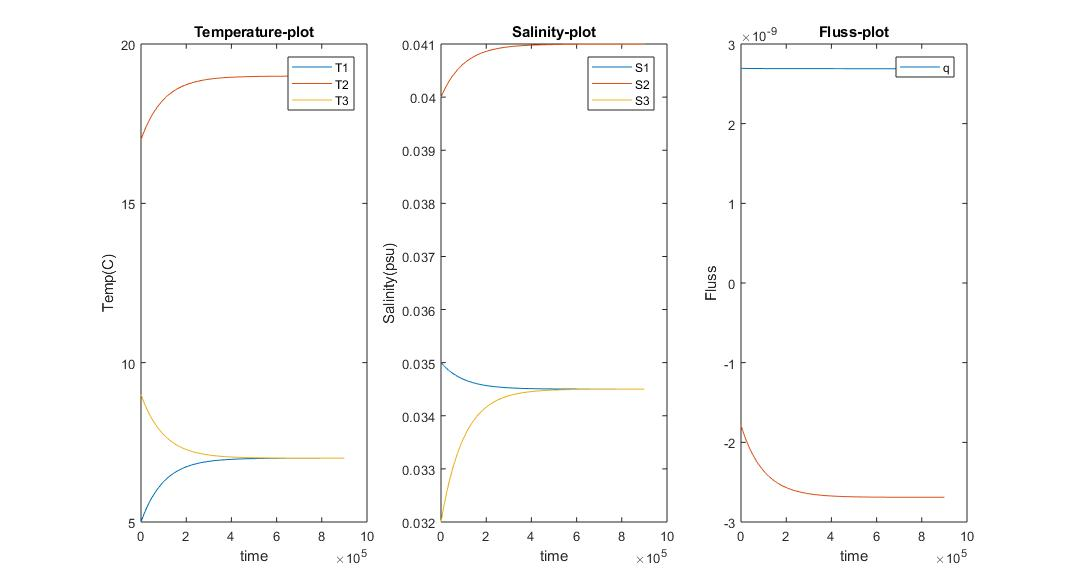
\includegraphics[width=14cm]{thermohalin/Code/graphs/result-3b2f-script.jpg}
	\centering
	\caption{Simulationsresultate}
	\label{thermohalin:simulationsresultate}
\end{figure}

Durch die Entkoppelung der zwei Flüsse, war es möglich, dass ein Fluss seine Richtung ändert.
Simulationstechnisch gesehen, hat das Modell funktioniert. Nur ist das Modell fehlerhaft. Das Modell muss also angepasst werden. Das Resultat der Anpassung ist in Abbildung \ref{thermohalin:3b2f-inverted} zu sehen.

\begin{figure}
	\centering
	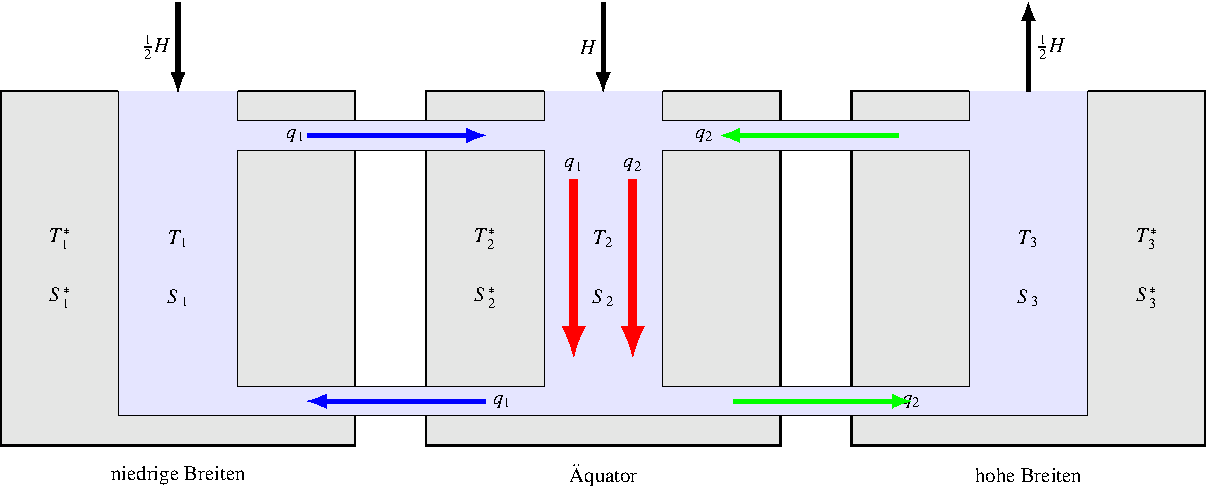
\includegraphics[width=14cm]{thermohalin/tikz/3b2f-inverted.pdf}
	\caption{Angepasstes Zwei-Fluss Modell}
	\label{thermohalin:3b2f-inverted}
\end{figure}

Nun lässt sich die neu entstandene Absinkstelle auch sofort erkennen. 
Mit diesem Modell lässt sich der Golfstrom also nicht erfolgreich simulieren. 
Der nächste, erfolgreichere, Ansatz wird im nächsten Abschnitt vorgestellt.

\subsection{Ein-Fluss Modell} 

Dieses Modell ist der verbesserte Nachfolger des Zwei-Fluss Modelles.
Es stammt aus einer Aufgabe von \texttt{Mathematics and Climate} \cite{skript:kaperengler}.

Um zu verhindern, dass in der mittleren Box eine zusätzliche Absinkzone entsteht, muss dieser Weg versperrt werden. Das erreicht man am einfachsten, wenn der Tiefenstrom von der Äquatorbox getrennt wird. Die Äquatorzone ist so nur via Oberflächenströmungen mit den anderen Boxen verbunden und die Tiefenströmung verbindet nur die Polzonen.


\begin{figure}
	\centering
	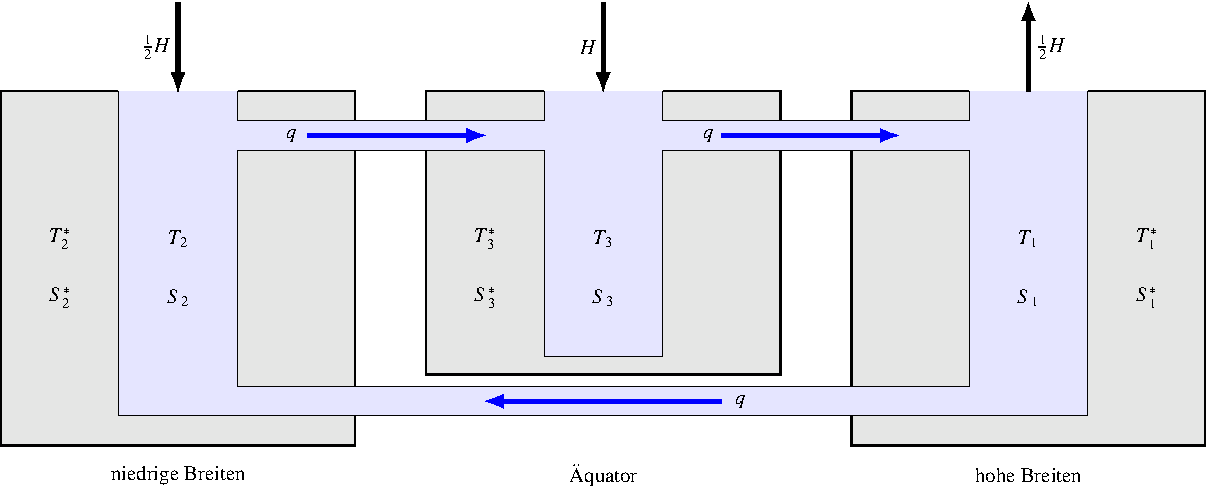
\includegraphics[width=14cm]{thermohalin/tikz/3b1f.pdf}
	\caption{Ein-Fluss Modell des THC}
	\label{thermohalin:3b1f}
\end{figure}

Wie im vorherigen Modell benötigen wir wieder 3 Gleichungen für Temperatur- und Salinitätsänderung der jeweiligen Boxen.
Jedoch gibt es nur noch einen Fluss welchen die Boxen verbindet. Das stimmt auch viel besser mit der Realität überein. Der Fluss wird nun von der Temperatur- und Salinitätsdifferenz zwischen der Betrachteten und der vorherigen Box getrieben. Folgend ist die Gleichung für für Box Nr. 1 dargestellt, um die Zusammenhänge zu erläutern:

\begin{equation}
\frac{dT_1}{dt} = c(T_p-T_1)+ \begin{cases} q(T_3-T_1)  \quad q>0 \\ |q|(T_2-T_1)  \quad q<0 \end{cases}
\end{equation}

Der erste Term beschreibt wie bisher den Temperaturaustausch zwischen Box und Umgebung. Der Zweite Term ist jedoch anders als vorher, da der Fluss je nach Flussrichtung von anderen Boxen getrieben wird. 
Wenn der Fluss positiv ist, also $q>0$, dann wird für die Berechnung Box Nr. 3 und die aktuelle Box verwendet, da die dritte Box die Quellbox darstellt. Wenn der Fluss nun negativ wird, ist die Quellbox jedoch Box Nr. 2 also muss hier Differenz zwischen der Zweiten und der Dritten Box berechnet werden. Um die Simulation zu erleichtern, wird im Falle eines negativen Flusses mit dem Absolutbetrag gerechnet. Damit die Resultate trotzdem stimmen werden  bei der Differenzbildung jeweils die Terme vertauscht damit die Richtung trotzdem stimmt. 

Das gesamte Gleichungssystem hat also folgende Form:

\begin{equation}
\begin{aligned}
\frac{dT_1}{dt} &= c(T_p-T_1)&+ \begin{cases} q(T_3-T_1) & \quad q>0 \\ |q|(T_2-T_1) & \quad q<0 \end{cases}
\\
\frac{dT_2}{dt} &= c(T_p-T_2)&+\begin{cases} q(T_1-T_2) & \quad q>0 \\ |q|(T_3-T_2) & \quad q<0 \end{cases}
\\
\frac{dT_3}{dt} &= c(T_e-T_3)&+\begin{cases} q(T_2-T_3) & \quad q>0 \\ |q|(T_1-T_3) & \quad q<0 \end{cases}
\end{aligned}
\end{equation}
\begin{equation}
\begin{aligned}
\frac{dS_1}{dt} &= -H/2 &+ d(S_p-S_1)&+\begin{cases} q(S_3-S_1) & \quad q>0 \\ |q|(S_2-S_1) & \quad q<0 \end{cases}
\\
\frac{dS_2}{dt} &= \phantom{-}H &+ d(S_p-S_2)&+\begin{cases} q(S_1-S_2) & \quad q>0 \\ |q|(S_3-S_2) & \quad q<0 \end{cases}	
\\
\frac{dS_3}{dt} &= -H/2 &+d(S_e-S_3)&+\begin{cases} q(S_2-S_3) & \quad q>0 \\ |q|(S_1-S_3) & \quad q<0 \end{cases}
\end{aligned}
\end{equation}	

Der Fluss $q$ wird weiter aus den Dichteunterschieden berechnet. Für die Berechnungen werden jedoch nur die polaren Boxen verwendet.

\begin{equation}
q = k[\alpha(T_1-T_3)-\beta(S_3-S_1)] 
\end{equation}

Aufgrund diese Gleichungen kann dann der neue Matlabcode geschrieben werden, welcher im nächsten Abschnitt erklärt wird.


\subsubsection{Matlab-code}

Die Übergabe der Startwerte und Konstanten, der Aufruf des Differentialgleichungslösers und das Plotten der Resultate sind gleich geblieben und werden deshalb nicht noch einmal gezeigt( \ref{thermohalin:listing:input}). Die Änderungen befinden sich in der Funktion selber. Je nachdem ob der Fluss positiv oder negativ ist muss ein anderer Fall der Gleichung berechnet werden. Dies wird mit einem \texttt{if}-Statement erreicht, welches in jedem Durchgang neu ausgewertet wird.

\lstinputlisting[style=Matlab]{thermohalin/listings/listing-3b1f-solve.m}






\subsubsection{Resultate} 

1. Resultat normale Simulation mit aktuellen Werten

2. Simulation der werte nach klimaerwärmung

3. Vergleich Paper Liu Wei


